\documentclass[a4paper]{article}

\usepackage[utf8]{inputenc}
\usepackage[T1]{fontenc,url}
\usepackage{hyperref}
\usepackage{amsmath, amssymb}
\usepackage{graphicx}
\usepackage{parskip}
\usepackage{lmodern}
\usepackage{algorithm}
\usepackage{algpseudocode}
\usepackage{epigraph}


\begin{document}
\title{FYS3150 -- Project 1}
\author{
    \begin{tabular}{r l}
        Kristian Gregorius Hustad & (\texttt{krihus})\\
        Jonas Gahr Sturtzel Lunde & (\texttt{jonassl})
    \end{tabular}}
%\date{}    % if commented out, the date is set to the current date

\maketitle

\setlength{\epigraphwidth}{0.7\textwidth}
\renewcommand{\epigraphflush}{center}
\renewcommand{\beforeepigraphskip}{70pt}
\renewcommand{\epigraphsize}{\normalsize}
\epigraph{The first principle is that you must not fool yourself -- and you are the easiest person to fool.}{\textit{Richard Feynman}}

\vfill

\begin{center}
    GitHub repository at \url{https://github.com/KGHustad/FYS3150}
\end{center}

\newpage

%%% MACROS
\newcommand{\half}{\frac{1}{2}}
\newcommand{\dx}{{\Delta x}}


\section{Introduction}
%\subsection*{Description of the nature of the problem}

In this project, we aim to find a numerical solution to the following ODE with Dirichlet boundary conditions
\begin{equation}
    -u''(x) = f(x), \quad x\in(0,1), \quad u(0) = u(1) = 0
    \label{eq:ddu_dxx_cont}
\end{equation}

\textbf{Her kan Jonas kanskje skrive noe om fysikken?}

\section{Discussion methods}
\subsection{An analytical solution}

With
\begin{equation}
    f(x) = 100e^{-10x}
\end{equation}

the analytical solution is given by
\begin{equation}
    u(x) = 1-(1-e^{-10})x-e^{-10x}
    \label{eq:u_analytical}
\end{equation}

We can easily check that \eqref{eq:u_analytical} is in fact a solution.

\begin{align*}
    \frac{d^2}{dx^2}  u(x)
    &= \frac{d^2}{dx^2} \left( 1-(1-e^{-10})x-e^{-10x} \right) \\
    &= \frac{d}{dx} \left( (1-e^{-10})+10e^{-10x} \right) \\
    &= -100e^{-10x} \\
    &= -f(x)
\end{align*}

\begin{figure}[ht]
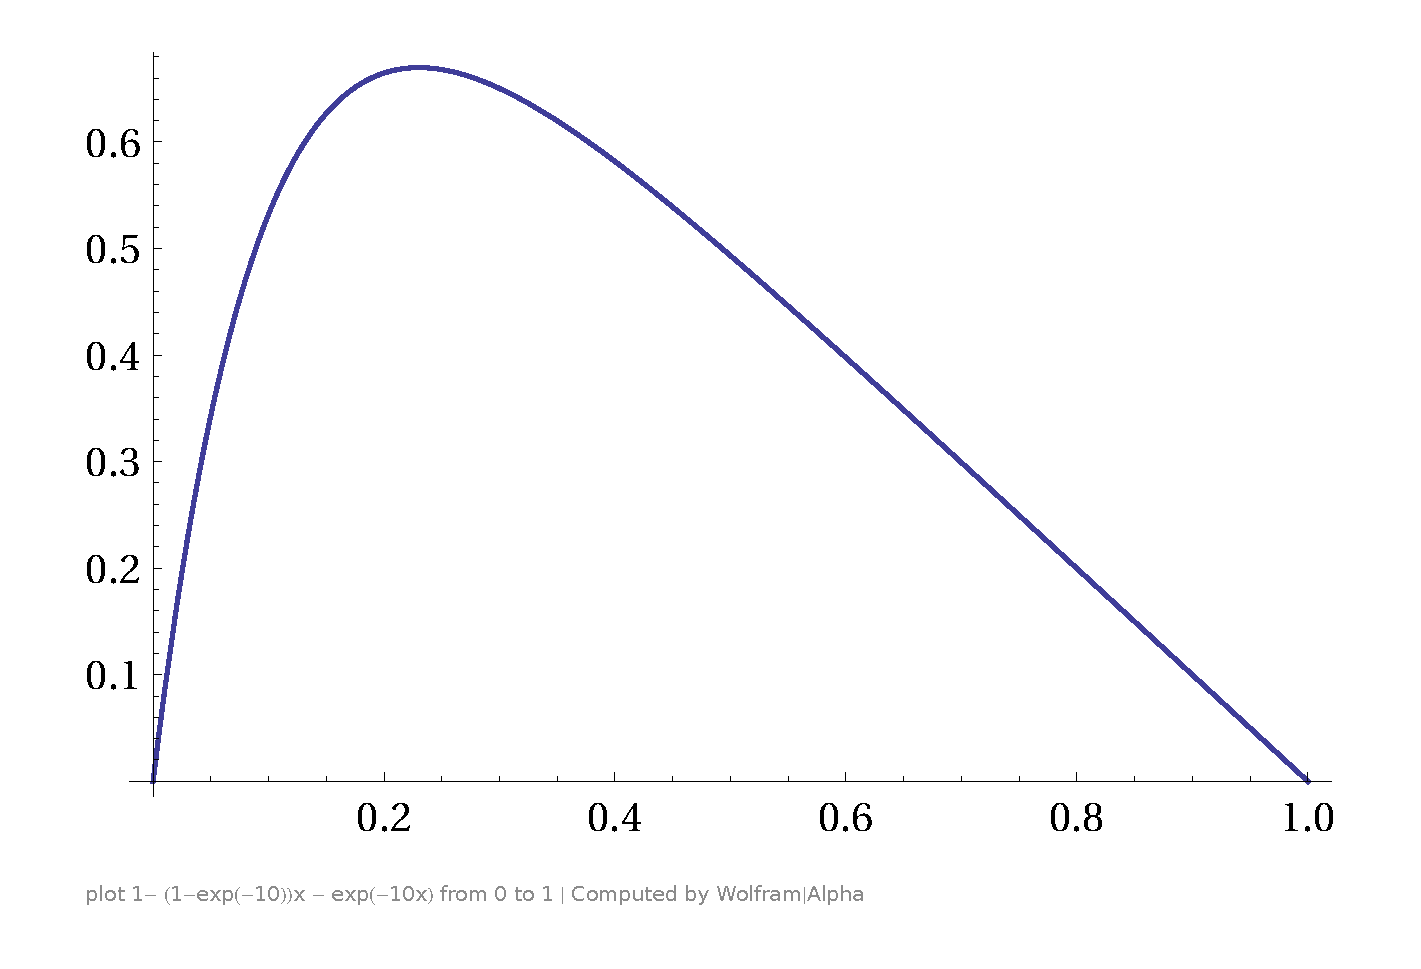
\includegraphics[width=\textwidth]{fig/exact_solution_wolfram_alpha_plot}
\caption{Plotting \eqref{eq:u_analytical} with Wolfram Alpha}
\end{figure}

\subsection{Deriving a numerical scheme}
Having reduced the problem to a purely mathematical one, we're left with the following ODE with Dirichlet boundary conditions
\begin{equation}
    -u''(x) = f(x), \quad x\in(0,1), \quad u(0) = u(1) = 0
    \label{eq:ddu_dxx_cont}
\end{equation}
where the source term, $f(x)$, is a known function.


We discretize $u(x), \quad x \in [0, 1]$ as $n+2$ ($n$ excluding the boundaries) equally spaced points $v_0, \dots, v_{n+1}$. To denote the set of indices for the points, we introduce $\mathcal{I} = \{ i \mid i \in \mathbb{Z}, 0 \leq i \leq n + 1\}$ and for the inner points (viz. excluding the boundaries) $\mathcal{I}_i = \{ i \mid i \in \mathbb{Z}, 0 < i < n + 1\}$.
The boundary conditions imply
\begin{equation}
v_0 = v_{n+1} = 0
\label{eq:boundaries_disc}
\end{equation}
The source term, $f(x), \quad x \in [0, 1]$ is discretized similarly. We can discretize \eqref{eq:ddu_dxx_cont} as

\begin{align*}
-[D_x D_x u]_i &= f_i \\
\frac{-1}{\dx} \left( [D_x u]_{i+\half} - [D_x u]_{i-\half} \right) &= f_i \\
\frac{-1}{\dx} \left( \frac{v_{i+1} - v_{i}}{\dx} - \frac{v_{i} - v_{i-1}}{\dx} \right) &= f_i \\
\frac{-1}{\dx^2} \left( v_{i+1} - 2v_{i} + v_{i-1} \right) &= f_i \\
-v_{i+1} + 2v_{i} - v_{i-1}  &= \dx^2 f_i
\end{align*}

where $i \in \mathcal{I}_i$. Setting $h = \dx$, we obtain the following equation

\begin{equation}
-v_{i+1} + 2v_{i} - v_{i-1}  = h^2 f_i, \quad i \in \mathcal{I}_i
\label{ddu_dxx_disc}
\end{equation}

This corresponds to a system of linear equations where the unknowns are $v_i, \quad i \in \mathcal{I}_i$. To save space, we introduce $s_i = h^2 f_i, i \in \mathcal{I}_i$.

\begin{equation}
    \begin{array}{cccc}
        a_1 v_{0} + b_1 v{1} + c_1 v_{2} &= s_1 \\
        a_2 v_{1} + b_2 v{2} + c_2 v_{3} &= s_2 \\
        \vdots \\
        a_n v_{n-1} + b_n v{n} + c_n v_{n+1} &= s_n \\
    \end{array}
\end{equation}

Being a system of linear equations, it can be rewritten as a matrix equation $A {\bf v} = {\bf s}$, where ${\bf v} = (v_1, \dots, v_{n})$, ${\bf s} = h^2 {\bf f} = (h^2 s_1, \dots, h^2 s_{n})$ and $A$ is a $n \times n$ matrix defined as below.

\begin{equation}
     A = \left(\begin{array}{ccccccccc}
                   b_1 & c_1 & 0 &\dots   & \dots &\dots & \dots &\dots&\dots\\
                   a_2 & b_2 & c_2 & 0 &\dots &\dots & \dots&\dots&\dots \\
                   0 & a_3 & b_3 & c_3 & 0 & \dots & \dots&\dots&\dots \\
                   \vdots&\vdots&\vdots&\vdots&\vdots&\vdots&\vdots&\vdots&\vdots \\
                   \dots&\dots&\dots&\dots&\dots & 0 & a_{n-1}  &b_{n-1}& c_{n-1} \\
                   \dots&\dots&\dots&\dots&\dots&\dots &  0 &a_n & b_n \\
              \end{array} \right)
\end{equation}

Notice that $a_1$ and $c_{n}$ does not appear in the matrix although they are present in the system of equations. As a consequence of the boundary conditions, we have \eqref{eq:boundaries_disc}, which in turn implies $a_1 v_{0} = a_1 \cdot 0 = 0$ and $c_n v_{n+1} = c_n \cdot 0 = 0$, hence we can omit $a_1$ and $c_{n}$ from the matrix.



\subsection{A general algorithm for solving an equation with a tridiagonal matrix}
We can solve $A {\bf v} = {\bf s}$ for any tridiagonal matrix $A$ with standard Gaussian elimination. Since most of the matrix elements are zero, we choose to represent the matrix as three arrays, \texttt{a}, \texttt{b}, and \texttt{c}.

\begin{algorithm}
\caption{Gaussian elimination for a tridiagonal matrix} \label{alg:gaussian-general-tridiagonal}
\begin{algorithmic}[1]
  \For {$i \gets 2, \dots, n$} \Comment{Forward substitution eliminating $a_i$}
    \State $b_i \gets b_i - c_{i-1}\cdot \frac{a_i}{b_{i-1}}$ \Comment{Update $b_i$}
    \State $s_i \gets s_i - s_{i-1}\cdot \frac{a_i}{b_{i-1}}$ \Comment{Update $s_i$}
    \State $a_i \gets a_i - b_{i-1}\cdot \frac{a_i}{b_{i-1}} = 0$ \Comment{Set $a_i$ to 0 (can be skipped)}
  \EndFor

  \Statex \Comment{Backward substitution obtaining $v_i$}
  \State $v_n \gets \frac{s_n}{a_n}$
  \For {$i \gets n-1, \dots, 1$}
    \State $v_i \gets \frac{s_i - b_i v_{i+1}}{a_i}$
  \EndFor
\end{algorithmic}
\end{algorithm}

\begin{figure}[ht]
\includegraphics[width=\textwidth]{fig/plot_b}
\caption{Approximation to $u$ by algorithm \ref{alg:gaussian-general-tridiagonal}}
\end{figure}


\subsection*{c) A more specialized algorithm}

\subsection*{d) Studying the error}

\subsection*{e) LU decomposition}


%\section{Results}




\end{document}
